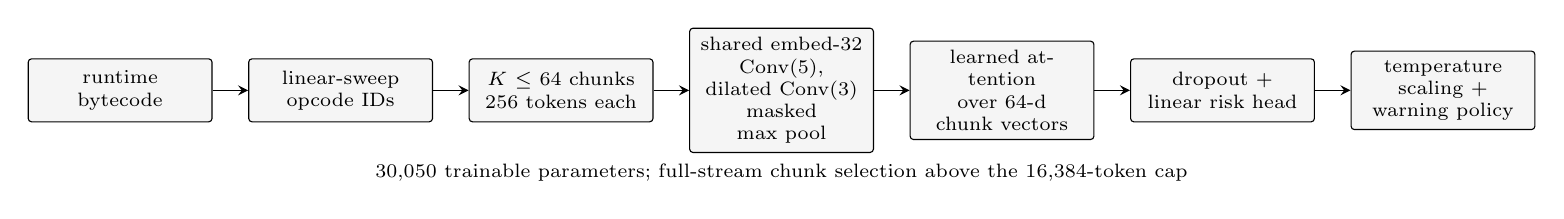
\begin{tikzpicture}[
  font=\scriptsize,
  box/.style={draw, rounded corners=1.2pt, minimum height=8mm, text width=21mm,
              align=center, fill=gray!8},
  flow/.style={->, >=stealth, line width=.6pt}
]
  \node[box] (bytecode) at (0,0) {runtime bytecode};
  \node[box] (tokens) at (2.8,0) {linear-sweep opcode IDs};
  \node[box] (chunks) at (5.6,0) {$K\leq64$ chunks\\256 tokens each};
  \node[box] (local) at (8.4,0) {shared embed-32\\Conv(5), dilated Conv(3)\\masked max pool};
  \node[box] (attn) at (11.2,0) {learned attention\\over 64-d chunk vectors};
  \node[box] (head) at (14.0,0) {dropout + linear risk head};
  \node[box] (policy) at (16.8,0) {temperature scaling + warning policy};
  \draw[flow] (bytecode) -- (tokens);
  \draw[flow] (tokens) -- (chunks);
  \draw[flow] (chunks) -- (local);
  \draw[flow] (local) -- (attn);
  \draw[flow] (attn) -- (head);
  \draw[flow] (head) -- (policy);
  \node[align=center] at (8.4,-1.05) {30,050 trainable parameters; full-stream chunk selection above the 16,384-token cap};
\end{tikzpicture}
